% Revised working manuscript for IJEPES.
% Author names, affiliations, correspondence, and repository URL remain placeholders.
\documentclass[final,5p,times]{elsarticle}

\usepackage{amsmath,amssymb,bm}
\usepackage{booktabs}
\usepackage{graphicx}
\usepackage{microtype}
\usepackage{xspace}
\usepackage{url}
\usepackage[hidelinks]{hyperref}
\usepackage{balance}
\usepackage{placeins}

\journal{International Journal of Electrical Power \& Energy Systems}
\urlstyle{same}
\emergencystretch=1em
\renewcommand{\bottomfraction}{0.80}
\renewcommand{\textfraction}{0.10}
\setcounter{bottomnumber}{2}
\raggedbottom

\newcommand{\method}{SGR--MACPO\xspace}

\begin{document}

\begin{frontmatter}

\title{Safety-Constrained Recurrent Multi-Agent Policy Optimization for Coupled Electricity--Hydrogen Scheduling in Multi-Microgrids}

\author[inst1]{Author Name 1}
\author[inst1]{Author Name 2}
\address[inst1]{Department of Electrical Engineering, Institution Name, City, Country}

\begin{abstract}
Coordinating multiple microgrids requires economic decisions to remain compatible with distribution-network voltage limits and with delayed hydrogen delivery. This paper proposes \method, a recurrent multi-agent constrained policy optimization method for electricity--hydrogen scheduling in four interconnected microgrids. Decentralized gated recurrent unit actors use local physical, market, inventory, and transportation observations, whereas centralized reward and voltage-cost critics are used only during training. The policy update combines reward and global voltage-cost natural-gradient directions within a Kullback--Leibler trust region and validates candidate parameters by sampled-cost backtracking. The environment couples continuous double-auction electricity and hydrogen markets, congestion-dependent hydrogen travel time, pending and late deliveries, emergency supply, and AC power flow on a native Swiss medium-voltage network. Across three deterministic day scenarios, \method reduced the accumulated raw voltage cost to 0.685, compared with 7.757 for unconstrained MAPPO and 1.409 for fixed-penalty MAPPO, while incurring a lower economic cost than the fixed-penalty controller. A same-checkpoint delivery-timing counterfactual further shows that explicit transport delay changes the in-transit inventory and the controller's physical hydrogen schedule.
\end{abstract}

\begin{keyword}
multi-microgrid \sep hydrogen \sep multi-agent reinforcement learning \sep constrained policy optimization \sep voltage security \sep energy management
\end{keyword}

\end{frontmatter}

\section{Introduction}
\label{sec:intro}

The joint use of renewable generation, batteries, electrolyzers, and hydrogen storage can increase the flexibility of local energy systems, but it also couples electricity operation to hydrogen conversion, inventory, trading, and delivery processes \cite{yue2021hydrogen,staffell2019hydrogen,parra2019hydrogen,li2023hierarchical}. Deterministic, stochastic, and robust optimization can explicitly represent device constraints and network-security limits and thereby provide model-grounded trading or scheduling solutions. Once AC power flow, energy conversion, dual-market clearing, and intertemporal inventories are modeled together, however, the resulting problem is typically nonlinear and nonconvex. Repeated online solution also becomes computationally demanding as the number of microgrids and decision variables increases. Under highly variable renewable generation, demand, and traffic conditions, stochastic and scenario-based formulations further require scenario generation, screening, or classification; their tractability and effectiveness depend on how well the selected scenarios cover actual operating conditions. These nonlinearities, online computational requirements, and complex uncertainties limit the practical scalability of conventional optimization.

Reinforcement learning can instead learn a direct mapping from observations to actions and, after training, execute decisions without resolving the complete scheduling model at every operating step \cite{he2025hydrogen}. Multi-agent reinforcement learning (MARL) is particularly suitable for multi-microgrids because each participant owns local assets and acts on local information, while peer-to-peer electricity and hydrogen trades couple their operating outcomes \cite{samadi2020decentralized,fang2021multiagent,zhang2023interconnected}. Conventional MARL, however, normally maximizes cumulative reward. Exploration and unconstrained policy updates can exchange distribution-network voltage security for local economic gains, because locally beneficial trades alter feeder injections and affect system-wide voltages \cite{paudel2019p2p,tushar2020p2p,sousa2019p2p,morstyn2018p2p}. Reward-only MARL is therefore insufficient for the network-security requirement considered here.

The present problem also contains partial observability caused by delayed hydrogen delivery: current tank inventory does not fully describe future available supply, because pending quantities, route congestion, and recent controls affect subsequent states. To address the combined need for fast decentralized decisions under uncertainty, representation of delayed logistics, and a global voltage-security constraint, this paper proposes \method for a four-microgrid electricity--hydrogen system. Recurrent actors retain the local temporal information needed to respond to delayed effects, centralized training represents system coupling that is unavailable during decentralized execution, and hourly AC-power-flow voltage violations are optimized as a separate cost. The algorithmic design is thus tailored directly to the dual-market, delayed-transport, and distribution-network-security characteristics of the studied system.

The main contributions are as follows:
\begin{enumerate}
  \item A multi-microgrid environment that couples electricity and hydrogen double auctions, delayed and lossy hydrogen transport, storage dynamics, emergency supply, and native Swiss medium-voltage AC power flow.
  \item \method, a shared-system adaptation of constrained multi-agent policy optimization with decentralized recurrent actors and centralized recurrent reward and voltage-cost critics.
  \item A practical policy update that combines reward and cost natural-gradient directions, invokes a conservative recovery direction for an infeasible sampled rollout, and checks candidate parameters by reward, cost, and Kullback--Leibler (KL) backtracking tests.
  \item An evaluation that separates economic cost and voltage security and uses same-checkpoint counterfactuals to expose the operational effect of delayed hydrogen delivery and recurrent information.
\end{enumerate}

\subsection{Background and related work}
\label{sec:related}

\paragraph{Reinforcement learning for power and multi-energy systems.}

Reinforcement learning has been studied for power-system operation, control, and demand response because it can learn sequential decisions from simulation or operational data \cite{glavic2017reinforcement,cao2020review,bahrami2021demand,vazquez2019demand,francois2018deep}. MARL extends this idea to systems with decentralized decision makers and coupled objectives. Samadi et al. \cite{samadi2020decentralized} developed decentralized reinforcement learning for microgrid energy management, Fang et al. \cite{fang2021multiagent} considered distributed microgrid-market strategies, and Zhang et al. \cite{zhang2023interconnected} addressed interconnected multi-energy microgrids. These studies establish the value of learned coordination, while the present work focuses on the interaction between delayed hydrogen logistics and AC-network voltage security.

Electricity--hydrogen scheduling is commonly formulated through deterministic, stochastic, or robust optimization. Hierarchical scheduling has been used to coordinate electricity and shared hydrogen energy \cite{li2023hierarchical}; system-level studies have also examined renewable-hydrogen economics and supply-chain infrastructure \cite{glenk2019economics,almansoori2009supply,moreno2017infrastructure}. Recent reinforcement-learning work has considered hydrogen-based industrial microgrids \cite{he2025hydrogen}. The distinguishing feature here is that matched hydrogen trades become in-transit physical states with route-dependent ETA, pending delivery, and terminal accounting, so the policy must reason about both market clearing and delivery completion.

\paragraph{Cooperative and safe multi-agent reinforcement learning.}

Centralized training with decentralized execution is widely used when agents act locally but share a system objective. Actor--critic, value-decomposition, and counterfactual methods provide important foundations for cooperative MARL \cite{lowe2017maddpg,sunehag2018vdn,rashid2020qmix,foerster2018coma}, while MAPPO shows that proximal policy optimization can be an effective cooperative baseline \cite{schulman2017ppo,yu2022mappo}. Reviews and benchmarks emphasize partial observability, non-stationarity, credit assignment, and evaluation sensitivity as recurring challenges \cite{gronauer2022survey,hernandez2019survey,oroojlooy2023review,papoudakis2021benchmark}.

Safety constraints require more than maximizing a scalar reward. Safe-reinforcement-learning surveys distinguish constrained optimization, recovery, shielding, and risk-sensitive approaches \cite{garcia2015safe}. Trust-region policy optimization provides the local policy geometry used by subsequent constrained methods \cite{schulman2015trpo}; CPO restricts the expected policy cost inside such a trust region \cite{achiam2017cpo}. Lyapunov, reward-constrained, and benchmark studies illustrate complementary safety formulations \cite{chow2018lyapunov,tessler2019reward,ray2019benchmark}, and MACPO extends constrained policy optimization to multi-agent settings \cite{gu2021macpo}. Safety-aware MARL has also been applied to network-constrained peer-to-peer energy trading \cite{ma2025network}. That line of work explicitly treats a shared distribution-network cost and illustrates why the policy update must account for the joint action rather than an isolated agent action. A related carbon-aware P2P framework combines continuous double auctions with a cooperative Markov game and trust-region policy learning \cite{liu2025carbon}. The present method follows the cost-aware trust-region principle but uses one system-level voltage cost, four recurrent actors, centralized recurrent critics, and a simultaneous update of the concatenated actor parameters. Recurrent policies are motivated by partial observability and delayed effects; recurrent Q-learning provides an early example of using gated memory to reconstruct decision-relevant history \cite{hausknecht2015drqn}.

\section{System model and problem formulation}
\label{sec:problem}

\begin{figure*}[t]
  \centering
  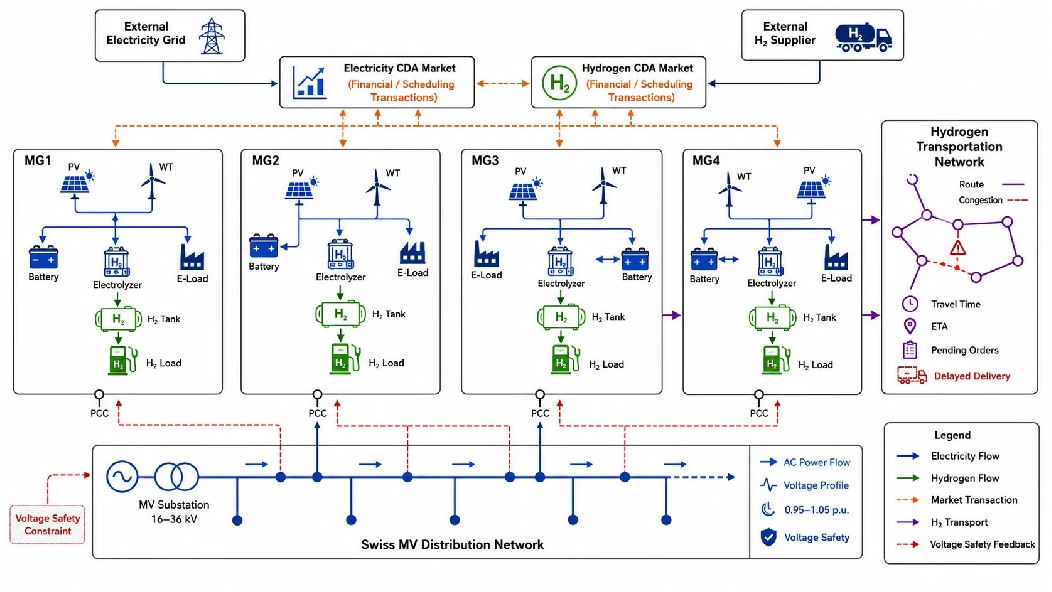
\includegraphics[width=0.96\textwidth]{fig_environment.pdf}
  \caption{Coupled electricity--hydrogen multi-microgrid environment. The electricity and hydrogen continuous double auctions (CDAs) determine financial and scheduling transactions; physical hydrogen is delivered through a congested transportation network, and each microgrid connects to the Swiss medium-voltage feeder through a point of common coupling (PCC).}
  \label{fig:environment}
\end{figure*}

\subsection{Constrained Markov game}

The system is modeled as a cooperative constrained Markov game with four agents. At time $t$, the joint state is $s_t$, agent $i$ receives local observation $o_t^i$, and selects continuous action $a_t^i$. The factorized joint policy is
\begin{equation}
  \boldsymbol{\pi}_{\boldsymbol{\theta}}(\boldsymbol{a}_t\mid\boldsymbol{o}_t)
  = \prod_{i=1}^{N}\pi_{\theta_i}(a_t^i\mid o_t^i,h_t^i),
  \qquad N=4,
\end{equation}
where $h_t^i$ is the hidden state of agent $i$'s gated recurrent unit (GRU) actor. The objective is the expected daily economic return
\begin{equation}
  \label{eq:daily_reward}
  J_R(\boldsymbol{\theta}) = \mathbb{E}_{\boldsymbol{\pi}_{\boldsymbol{\theta}}}
  \left[\sum_{t=0}^{T-1} r_t\right], \qquad T=24,
\end{equation}
subject to the global voltage-cost constraint
\begin{equation}
  J_C(\boldsymbol{\theta}) = \mathbb{E}_{\boldsymbol{\pi}_{\boldsymbol{\theta}}}
  \left[\sum_{t=0}^{T-1} c_t\right] \leq d.
\end{equation}

The environment returns a raw voltage cost $c_t^{\mathrm{raw}}$. The critic target is normalized as
\begin{equation}
  \label{eq:normalized_cost}
  c_t = \frac{c_t^{\mathrm{raw}}}{0.02}, \qquad d=1.0,
\end{equation}

\subsection{Microgrid assets, observations, and actions}

Each microgrid contains photovoltaics (PV), wind turbines (WT), a battery, an electrolyzer, a hydrogen tank, electric demand, and hydrogen demand. Table~\ref{tab:assets} lists the heterogeneous asset capacities used in the experiments.

\begin{table*}[t]
\centering
\caption{Asset capacities of the four microgrid agents. Battery energy is in kWh, hydrogen tank capacity is in kg, and hydrogen charge/discharge power is expressed as the lower-heating-value energy equivalent.}
\label{tab:assets}
\small
\begin{tabular}{lrrrrrrr}
\toprule
Agent & PV (kW) & WT (kW) & Battery (kWh) & Battery power (kW) & Electrolyzer (kW) & H$_2$ tank (kg) & H$_2$ tank power (kW$_{\mathrm{H2}}$)\\
\midrule
MG1 & 5000 & 1000 & 5000 & 2000 & 2000 & 500 & 2000\\
MG2 & 1000 & 4000 & 3000 & 1200 & 3000 & 500 & 2000\\
MG3 &  500 & 3000 & 4000 & 1500 &  500 & 300 & 1200\\
MG4 & 2000 &  500 & 2000 &  800 &  800 & 300 & 1500\\
\bottomrule
\end{tabular}
\end{table*}

The local base observation contains 32 normalized features describing renewable generation and load, battery state of charge, hydrogen inventory, recent market prices and exchanges, time encoding, pending-arrival buckets, tank headroom, route conditions, and local hydrogen-supply facts. Appending the agent's previous seven-dimensional action produces a 39-dimensional actor input. No instantaneous cross-agent transaction broadcast is supplied at execution time.

The action vector is
\begin{equation}
 a_t^i=[a_{\mathrm{el}},a_{\mathrm{bat}},a_{\mathrm{e,bid}},a_{\mathrm{h,bid}},
 a_{\mathrm{tank}},a_{\mathrm{h,buy}},a_{\mathrm{route}}]^{\top}.
\end{equation}
Its components control electrolyzer power, signed battery power, electricity bid price, hydrogen bid price, signed hydrogen-tank power, forward hydrogen buy quantity, and route selection, respectively.

\subsection{Electricity and hydrogen markets}

Electricity orders are formed from the physical net electric demand and cleared through a continuous double auction. Residual deficits or surpluses are balanced by the external grid. Hydrogen orders are cleared through an analogous market. When delivery lag is active, an internally matched hydrogen trade is financially recorded at clearing time, while its physical quantity enters a pending-delivery queue according to the selected route. The portion of a hydrogen buy order that is not filled by internal sellers becomes a regular external-supplier order and reaches the tank only after transportation. If physically available hydrogen remains insufficient for the current load, emergency hydrogen is then purchased for immediate balancing. Regular external orders provide intertemporal replenishment, whereas emergency purchases cover the current-hour shortfall; the two quantities are accounted for separately.

The transportation module contains four microgrid nodes and an external supplier node. Each shipment selects one of three candidate routes. Reproducible background traffic has morning and evening peaks, and route ETA is calculated from a bounded Bureau of Public Roads congestion model. The evaluated configuration produces an approximate 4--10 h ETA range and includes in-transit loss. Hydrogen that has not entered a local tank by the episode boundary has zero terminal asset value.

\subsection{Physical state transitions and balances}
\label{sec:physical_transitions}

The environment retains the physical states that connect market decisions across hours. Let $\Delta t$ denote the one-hour step, and define $P_{i,t}^{\mathrm{bat},+}=\max(P_{i,t}^{\mathrm{bat}},0)$ and $P_{i,t}^{\mathrm{bat},-}=\max(-P_{i,t}^{\mathrm{bat}},0)$. The battery state of charge is updated as
\begin{equation}
  \label{eq:soc_transition}
  \begin{aligned}
  \mathrm{SOC}_{i,t+1}=\operatorname{clip}\!\bigg(&\mathrm{SOC}_{i,t}+
  \frac{\eta_{i,c}^{\mathrm{bat}}P_{i,t}^{\mathrm{bat},+}-P_{i,t}^{\mathrm{bat},-}/\eta_{i,d}^{\mathrm{bat}}}{E_i^{\mathrm{bat},\max}}\Delta t,\\[-1mm]
  &\mathrm{SOC}_i^{\min},\mathrm{SOC}_i^{\max}\bigg).
  \end{aligned}
\end{equation}
The action-dependent power limits are applied before this update, so the SOC remains within its physical range. Electrolyzer power is converted to hydrogen energy according to
\begin{equation}
  \label{eq:electrolyzer_transition}
  E_{i,t}^{\mathrm{H2,prod}}=\eta_i^{\mathrm{el}}P_{i,t}^{\mathrm{el}}\Delta t,
  \qquad
  E_{i,t}^{\mathrm{H2,load}}=\frac{\sigma_i L_{i,t}^{\mathrm{H}}\Delta t}{\eta^{\mathrm{boiler}}},
\end{equation}
where $\sigma_i$ is the hydrogen share of the thermal demand. For tank power, positive values denote charging and negative values denote discharging. With $P_{i,t}^{\mathrm{tank},+}$ and $P_{i,t}^{\mathrm{tank},-}$ defined analogously, the tank inventory in kg follows
\begin{equation}
  \label{eq:h2_tank_transition}
  H_{i,t+1}=\operatorname{clip}\!\left(H_{i,t}+
  \frac{\eta_{i,c}^{\mathrm{H2}}P_{i,t}^{\mathrm{tank},+}-P_{i,t}^{\mathrm{tank},-}/\eta_{i,d}^{\mathrm{H2}}}{\mathrm{LHV}_{\mathrm{H2}}}\Delta t,\,
  H_i^{\min},H_i^{\max}\right).
\end{equation}

For each matched hydrogen trade, the delivered quantity is reduced by the route loss and inserted into a pending-arrival queue indexed by its ETA. If $q_{i,t}(\ell)$ is the hydrogen energy scheduled to arrive at microgrid $i$ after $\ell$ hours, the queue evolves conceptually as
\begin{equation}
  \label{eq:pending_transition}
  \begin{aligned}
  q_{i,t+1}(\ell-1)&=q_{i,t}(\ell),\quad \ell\geq1,\\[-1mm]
  q_{i,t+1}(\mathrm{ETA}_{ij,t})&\mathrel{+}=(1-\xi_{ij,t})q_{ij,t}^{\mathrm{clear}}.
  \end{aligned}
\end{equation}
where $\xi_{ij,t}$ is the route-dependent loss fraction. The $\ell=0$ arrivals are added to the receiving tank before the next tank-power clipping operation. Thus, a cleared transaction is financially settled at the current hour but becomes physically available only at its arrival time.

The resulting local balances passed to the two CDAs are
\begin{align}
  P_{i,t}^{\mathrm{net,e}} &= L_{i,t}^{\mathrm{e}}+P_{i,t}^{\mathrm{el}}+P_{i,t}^{\mathrm{bat},+}-P_{i,t}^{\mathrm{PV}}-P_{i,t}^{\mathrm{WT}}-P_{i,t}^{\mathrm{bat},-},\label{eq:electric_balance}\\
  E_{i,t}^{\mathrm{net,H2}} &= E_{i,t}^{\mathrm{H2,load}}+P_{i,t}^{\mathrm{tank}}\Delta t-E_{i,t}^{\mathrm{H2,prod}}.\label{eq:h2_balance}
\end{align}
Positive net quantities represent purchases and negative quantities represent available surplus. The CDA clears internal orders, while residual quantities are balanced through the corresponding external market. These transitions make the delayed logistics state explicit without introducing a generic Markov transition matrix.

\subsection{Distribution-network power flow and safety cost}

The selected Swiss-PDGs case is network 347\_1, with PCC buses [168, 147, 160, 183], native 20-kV medium-voltage data, and a 100-MVA base \cite{swisspdgs}. At every environment step, microgrid PCC active and reactive injections are added to the network case and solved by Newton--Raphson AC power flow using a MATPOWER-compatible formulation \cite{zimmerman2011matpower}. For bus voltage $V_{n,t}$, the raw voltage cost is
\begin{equation}
 c_t^{\mathrm{raw}}=\sum_{n}\left[\max(0,0.95-V_{n,t})
 +\max(0,V_{n,t}-1.05)\right].
\end{equation}
A failed power flow is assigned a cost of 1.0. The constrained quantity in this study is the system-level voltage cost.

\section{Proposed SGR--MACPO method}
\label{sec:method}

The formulation in Section~\ref{sec:problem} combines continuous market actions, nonlinear AC-network responses, delayed state transitions, and decentralized observations. A centralized online optimizer would require information that is not available to each microgrid at execution time, whereas an unconstrained MARL update would not directly control the voltage cost in~\eqref{eq:normalized_cost}. We therefore use centralized training with decentralized recurrent execution and adapt constrained policy optimization to one shared system-level safety cost. The recurrent architecture addresses delayed and partially observed consequences; the separate cost critic estimates network risk; and the trust-region recovery and acceptance tests restrict policy changes when the sampled rollout is infeasible.

\subsection{Centralized training and recurrent actors}

The execution policy is decentralized. Agent $i$ receives only $o_t^i$, its previous action, and its recurrent hidden state. The GRU summarizes recent control, inventory, and delivery information that cannot be inferred from a single instantaneous measurement. During training, the four local observations are concatenated for a centralized reward critic $V_R$ and a centralized voltage-cost critic $V_C$, allowing both critics to evaluate the joint effect of otherwise local actions. Generalized advantage estimation is applied separately to the dense hourly reward and normalized voltage-cost trajectories; its numerical settings are reported in Table~\ref{tab:training_parameters}.

\subsection{Reward and cost surrogate objectives}

Let $\hat A_R$ and $\hat A_C$ denote reward and cost advantages. For candidate actor parameters $\theta$, the first-order episode-sum surrogate is
\begin{equation}
 L_X(\theta)=\mathbb{E}_{\mathrm{env}}\left[
 \sum_{t=0}^{T-1}\sum_{i=1}^{N}
 \left(\rho_t^i(\theta)-1\right)\hat A_X(t)\right],
 \quad X\in\{R,C\},
\end{equation}
where $\rho_t^i$ is the action-probability ratio. The sampled cost estimate is
\begin{equation}
 \widetilde J_C(\theta)=\bar C+L_C(\theta).
\end{equation}
The episode-sum form is necessary because averaging over time and agents would understate the daily cost response by approximately $TN=96$ in this configuration.

\subsection{Trust-region geometry}

The method computes reward gradient $g_R$, cost gradient $g_C$, and the Hessian of the average KL divergence. The Fisher-vector product is evaluated implicitly as
\begin{equation}
  \label{eq:fisher_vector_product}
  Fv = H_{\mathrm{KL}}v+\eta v,
\end{equation}
where $\eta$ is a damping coefficient. Conjugate gradients approximate $F^{-1}g_R$ and $F^{-1}g_C$. When the sampled rollout exceeds the cost budget, \method enters a conservative recovery branch and chooses a cost-reducing direction. When the rollout is feasible, it uses the reward direction unless the linearized cost would cross the budget; in that case, the direction is formed on the intersection of the linearized cost boundary and the KL ellipsoid. Candidate parameters are accepted only after backtracking if they satisfy the KL limit and the applicable reward and cost tests. This sequence directly links the voltage constraint to the actor update instead of selecting a fixed scalar trade-off between reward and cost. Numerical update settings are given in Table~\ref{tab:training_parameters}.

\subsection{Feasible and recovery directions}
\label{sec:update_directions}

Let $\Delta\boldsymbol{\theta}$ denote a simultaneous update of the concatenated actor parameters, let $c_0=\widetilde J_C(\boldsymbol{\theta})-d$ be the sampled cost gap, and define
\begin{equation}
  \label{eq:local_constrained_update}
  \max_{\Delta\boldsymbol{\theta}}\; g_R^{\top}\Delta\boldsymbol{\theta}
  \quad\mathrm{s.t.}\quad c_0+g_C^{\top}\Delta\boldsymbol{\theta}\leq0,\qquad
  \frac{1}{2}\Delta\boldsymbol{\theta}^{\top}F\Delta\boldsymbol{\theta}\leq\delta.
\end{equation}
The two natural-gradient coordinates are $u_R=F^{-1}g_R$ and $u_C=F^{-1}g_C$, obtained by conjugate gradients using the Fisher-vector product in~\eqref{eq:fisher_vector_product}. Define
\begin{equation}
  q_R=g_R^{\top}u_R,\qquad q_C=g_C^{\top}u_C,\qquad q_{RC}=g_R^{\top}u_C.
\end{equation}
If $c_0>0$ and $q_C>0$, the sampled rollout is updated in the cost-recovery direction
\begin{equation}
  \label{eq:recovery_direction}
  \Delta\boldsymbol{\theta}_{\mathrm{rec}}=-\sqrt{\frac{2\delta}{q_C}}\,u_C.
\end{equation}
For a feasible rollout, the unconstrained reward direction is $\Delta\boldsymbol{\theta}_R=\sqrt{2\delta/q_R}\,u_R$. It is retained when $c_0+g_C^{\top}\Delta\boldsymbol{\theta}_R\leq0$. Otherwise, the update is placed on the intersection of the linearized cost boundary and the KL ellipsoid. With
\begin{equation}
  r_\delta=2\delta-\frac{c_0^2}{q_C},\qquad
  q_\perp=q_R-\frac{q_{RC}^2}{q_C},
\end{equation}
the constrained direction is
\begin{equation}
  \label{eq:intersection_direction}
  \Delta\boldsymbol{\theta}_{\mathrm{con}}=\alpha u_R+\beta u_C,\qquad
  \alpha=\sqrt{\frac{r_\delta}{q_\perp}},\qquad
  \beta=\frac{-c_0-\alpha q_{RC}}{q_C},
\end{equation}
whenever the denominators and the residual KL radius are positive. These equations describe the implementation-level shared-system adaptation: all four recurrent actors are updated together using one voltage-cost gradient, rather than using the sequential per-agent decomposition of other multi-agent safe-policy methods.

\subsection{Sampled-cost backtracking}
\label{sec:backtracking}

For a selected direction $\Delta\boldsymbol{\theta}$, candidate parameters are generated as
\begin{equation}
  \label{eq:backtracking_candidate}
  \boldsymbol{\theta}^{(k)}=\boldsymbol{\theta}+\zeta^k\Delta\boldsymbol{\theta},qquad
  k=0,\ldots,K-1,
\end{equation}
where $\zeta=0.5$ and $K=10$ in the reported experiments. Each candidate is evaluated with the sampled reward surrogate, sampled voltage-cost objective, and average KL divergence. A recovery candidate is accepted when its sampled cost does not exceed the current sampled cost and its KL divergence is within $\delta$; a reward or constrained-reward candidate must additionally satisfy the sampled cost budget and must not reduce the sampled reward. The first candidate satisfying these tests is applied. This explicit acceptance step prevents the linearized surrogate from being the sole safety check.

The resulting update flow is: collect recurrent trajectories; fit the centralized reward and voltage-cost critics; compute separate advantages and gradients; solve the implicit Fisher systems; select reward, constrained-reward, or recovery direction; and apply sampled-cost backtracking. The compact flow is also summarized in Fig.~\ref{fig:algorithm}.

\begin{figure}[t]
  \centering
  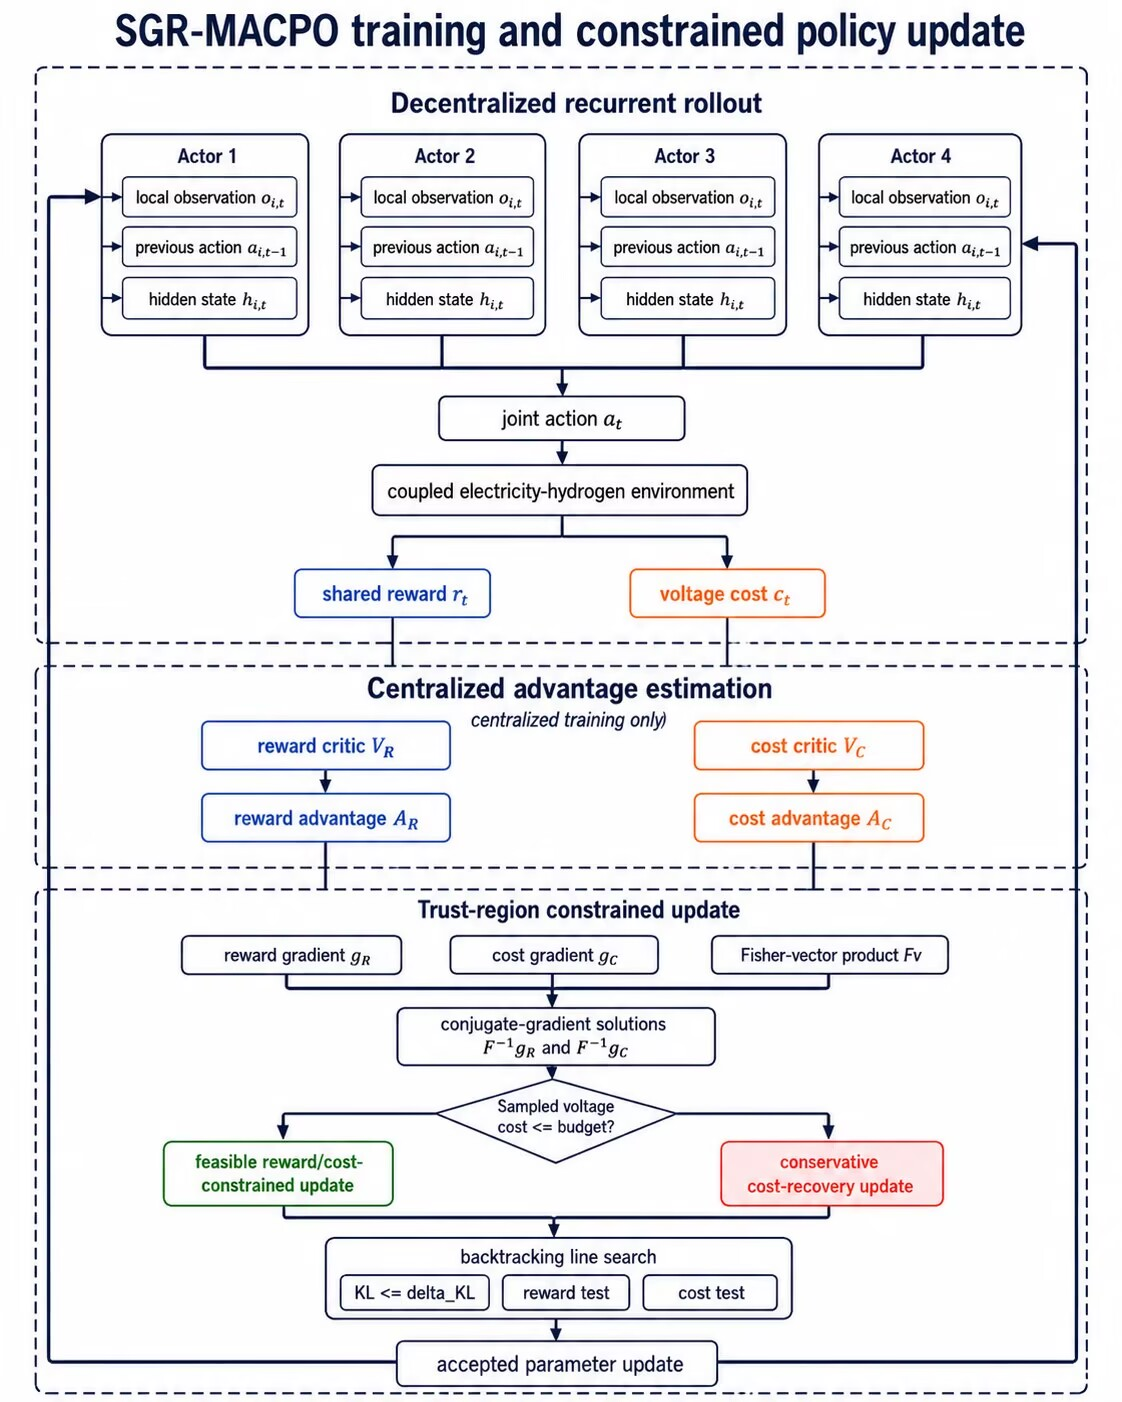
\includegraphics[width=0.98\columnwidth]{fig_algorithm_image2.png}
  \caption{Training and constrained policy-update workflow of \method. Decentralized recurrent actors interact with the coupled environment, while reward and voltage-cost critics are centralized during training. Feasible and recovery updates are screened by KL, reward, and cost tests during backtracking.}
  \label{fig:algorithm}
\end{figure}

\section{Case studies and results}
\label{sec:experiments}

\subsection{Evaluation protocol and metrics}

The main operating comparison uses three reproducible deterministic evaluation-day and traffic scenarios. The compared methods are unconstrained MAPPO, fixed-penalty MAPPO, and \method. They share the same environment, observations, action space, and GRU actor--critic architecture and differ primarily in their policy updates. A Lagrangian controller is used only in the training-curve diagnostic and is not included in the three-day operating table.

The case studies answer four questions that correspond to the proposed contributions: (i) whether the constraint-aware update improves the voltage--economy balance; (ii) how electricity-CDA clearing propagates through residual grid exchange to the voltage trajectory; (iii) how the hydrogen CDA and regular external orders affect closed-loop operation through delayed delivery; and (iv) whether the recurrent actor uses its temporal inputs. Economic performance is reported as accumulated operating cost in million CNY, while network performance is reported through raw voltage cost, minimum bus voltage, and the hourly violation profile.

Table~\ref{tab:training_parameters} summarizes the main training and update parameters. The choice $\gamma=1$ matches the undiscounted 24-h scheduling objective, and the \method actor follows the constrained natural-gradient update.

\begin{table}[t]
\centering
\caption{Training and update parameters used in the reported Env-v6 comparison. Method-specific settings are identified explicitly.}
\label{tab:training_parameters}
\scriptsize
\setlength{\tabcolsep}{4.0pt}
\begin{tabular}{ll}
\toprule
Setting & Value\\
\midrule
GRU hidden size (actor/critics) & 128\\
Actor input dimension & 39\\
Parallel environments $\times$ horizon & $2\times24$\\
Training updates & 1000\\
Discount $\gamma$ / GAE $\lambda$ & 1.0 / 0.95\\
Adam learning rate & $3\times10^{-4}\!\rightarrow0$\\
MAPPO clip / entropy coefficient & 0.2 / 0.01\\
Penalty-MAPPO cost coefficient $\alpha$ & 1.0\\
SGR--MACPO raw/normalized budget & 0.02 / 1.0\\
SGR--MACPO KL / CG / damping & 0.01 / 10 / $10^{-2}$\\
SGR--MACPO backtracks / ratio & 10 / 0.5\\
\bottomrule
\end{tabular}
\end{table}

\begin{table}[t]
\centering
\caption{Three-day deterministic Env-v6 evaluation from one trained policy per method. All controllers use GRU policies.}
\label{tab:main_results}
\scriptsize
\setlength{\tabcolsep}{3.2pt}
\begin{tabular}{lcc}
\toprule
Method & Voltage cost & Cost (M CNY)\\
\midrule
MAPPO & 7.757 & 2.94\\
Fixed-penalty MAPPO & 1.409 & 23.53\\
\method & 0.685 & 11.90\\
\bottomrule
\end{tabular}
\end{table}

\begin{figure}[t]
  \centering
  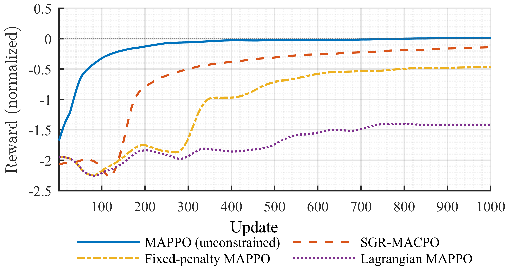
\includegraphics[width=0.98\columnwidth]{fig_convergence_reward.pdf}
  \caption{Scaled training-reward trajectories for the compared algorithms. The curves are separated from the voltage-cost trajectories so that the safety--economy trade-off remains legible at single-column width.}
  \label{fig:reward_convergence}
\end{figure}

\begin{figure}[t]
  \centering
  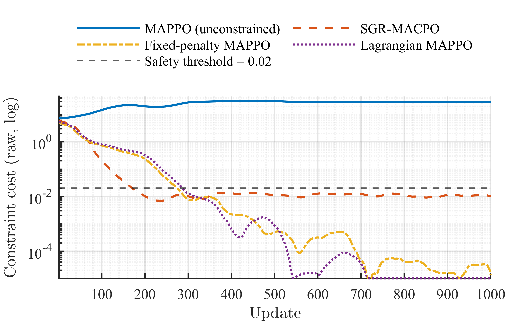
\includegraphics[width=0.98\columnwidth]{fig_convergence_voltage_cost.pdf}
  \caption{Raw training voltage-cost trajectories on a logarithmic scale. The dashed horizontal line denotes the raw daily voltage-cost budget of 0.02.}
  \label{fig:cost_convergence}
\end{figure}

\FloatBarrier
\subsection{Overall performance}
\label{sec:results}

The unconstrained MAPPO baseline obtains the lowest economic cost in Table~\ref{tab:main_results}, but it produces the largest voltage violation. Fixed-penalty MAPPO reduces violations at the expense of a markedly larger economic cost, illustrating the sensitivity of a fixed reward--cost weight. \method reduces the accumulated three-day raw voltage cost by 91.2\% relative to MAPPO and by 51.4\% relative to fixed-penalty MAPPO, while retaining a lower economic cost than the latter.

The convergence curves in Figs.~\ref{fig:reward_convergence} and \ref{fig:cost_convergence} separate the economic and safety objectives. Unconstrained MAPPO reaches the highest reward but remains above the voltage-cost budget. \method converges to a lower reward while reducing the cost signal, whereas fixed-penalty and Lagrangian updates obtain lower cost with a larger economic sacrifice. This behavior represents a safety--economy trade-off rather than reward dominance.

\subsection{Electricity-CDA-mediated network-security case}
\label{sec:cda_network_case}

The CDA is the link between decentralized actions and the network-security cost. At each hour, an actor first determines local device operation and the resulting physical net electricity and hydrogen demand, together with bid prices and quantities. The electricity CDA then matches internal sellers and buyers by price--time priority; only residual deficits or surpluses are settled with the external grid. The hydrogen CDA follows the same market logic, but a matched hydrogen quantity is financially cleared immediately and enters the physical delivery queue according to its route-dependent ETA.

\begin{figure}[t]
  \centering
  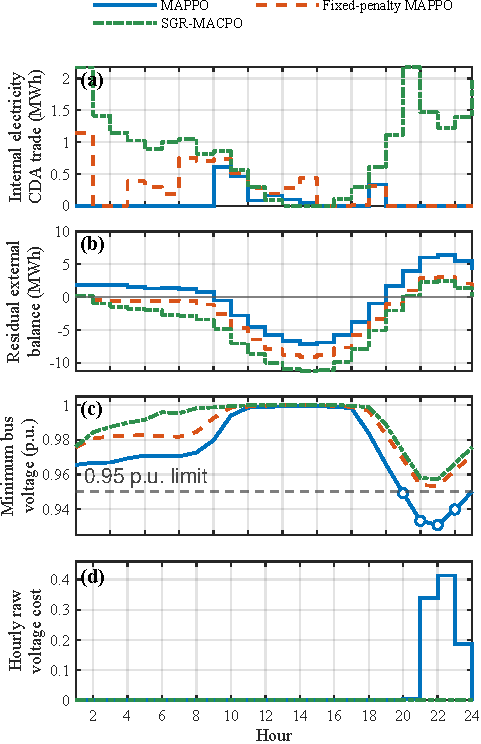
\includegraphics[width=0.98\columnwidth]{fig_voltage_case_seed32.pdf}
  \caption{Electricity-CDA-to-network chain in the representative scenario: (a) internal CDA trade; (b) residual external balance after clearing (positive for import); (c) minimum feeder-bus voltage; and (d) raw voltage cost. Open circles mark MAPPO low-voltage hours.}
  \label{fig:voltage_case}
\end{figure}

Fig.~\ref{fig:voltage_case} makes the market-to-network chain explicit for the representative scenario. Over the day, \method clears 21.66~MWh internally, versus 1.80~MWh for MAPPO and 6.24~MWh for fixed-penalty MAPPO. During the critical hours 20--24, it clears 8.22~MWh internally and leaves 6.44~MWh of residual imports; the two baselines clear no internal electricity trade and require 26.21 and 15.82~MWh, respectively. MAPPO consequently falls below 0.95~p.u. during hours 20--23, reaches 0.9309~p.u., and accumulates a raw voltage cost of 0.943. Fixed-penalty MAPPO and \method remain above the limit, with minima of 0.9533 and 0.9572~p.u. and zero voltage cost. Since CDA rules, environment, recurrent architecture, observations, and actions are shared, these market-clearing and residual-balance patterns are consequences of the policies learned under the different updates. The separate system-voltage cost direction in \method therefore supports active evening-peak internal coordination while keeping the residual PCC exchange on a voltage-safe trajectory.

The four panels also reveal three operating regimes. During hours 1--8, \method keeps internal CDA volume between 0.82 and 2.17~MWh while the two baselines mostly clear little or no electricity internally; its residual balance therefore moves from a small import to a moderate export instead of remaining a sustained import. During hours 9--18, the residual balance becomes negative for all methods as local generation exceeds aggregate demand. The internal-trade curves simultaneously contract toward zero around hours 13--15, which is consistent with a period in which the order books have insufficient buy--sell overlap and the remaining surplus is exported externally. The important separation appears again after hour 19: MAPPO's residual import rises from 1.72 to 6.46~MWh and its minimum voltage falls from 0.9659 to 0.9309~p.u.; fixed-penalty MAPPO limits the import to 3.10~MWh at hour 22; \method uses 1.11--2.18~MWh of internal CDA trade during hours 19--24 and keeps the residual import below 2.45~MWh. This hour-aligned comparison is the operating signature expected from a system-level voltage-cost direction: the policy changes which local surpluses serve which local deficits before the remaining imbalance reaches the PCC. As emphasized in network-constrained P2P safety analysis~\cite{ma2025network}, the relevant evidence is therefore not only the final voltage value but also the change in the trading pattern that precedes it.

\subsection{Hydrogen CDA and delivery-timing counterfactual}

\begin{figure}[t]
  \centering
  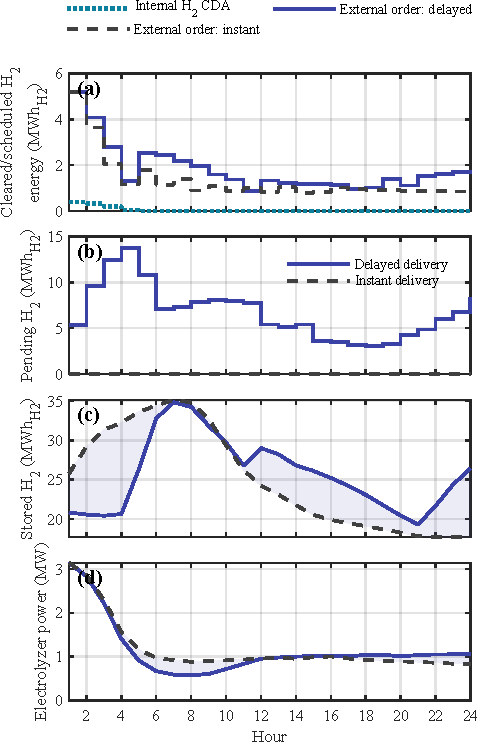
\includegraphics[width=0.98\columnwidth]{fig_h2_delay_case_seed32_singlecol.pdf}
  \caption{Hydrogen-market-to-delivery chain under delayed and instantaneous delivery in the representative scenario: (a) internally cleared hydrogen-CDA energy and regular external orders; (b) pending in-transit energy; (c) stored hydrogen; and (d) electrolyzer power. Only physical delivery timing is changed; the checkpoint and observation dimensions are preserved.}
  \label{fig:h2_delay_case}
\end{figure}

To isolate delivery timing, the same \method checkpoint is evaluated in closed loop with congestion-dependent and instantaneous delivery, without retraining. At each hour, the hydrogen CDA first clears internal buy and sell orders; any unfilled buy quantity becomes a regular external-supplier order. Both internal trades and regular external orders pass through the transport queue in the delayed case and arrive immediately in the counterfactual. The internal hydrogen CDA clears 0.96~MWh$_{\mathrm{H2}}$ in both trajectories, while delay raises regular external orders from 31.8 to 43.4~MWh$_{\mathrm{H2}}$. The resulting in-transit inventory changes stored hydrogen and shifts electrolyzer operation: power is lower during hours 5--10 but higher during hours 19--24. Emergency supply is 43.2 versus 32.1~MWh$_{\mathrm{H2}}$, and 8.38~MWh$_{\mathrm{H2}}$ remains pending at the delayed-case boundary versus zero under instantaneous delivery.

The direction changes in Fig.~\ref{fig:h2_delay_case} are physically interpretable. In hours 1--4, the delayed case accumulates pending energy to 13.78~MWh$_{\mathrm{H2}}$ while the instantaneous case has no queue; the delayed controller consequently operates the electrolyzer below the instantaneous trajectory during hours 5--10, when earlier shipments begin arriving and temporarily replenish the tank. From hours 12--20, the delayed pending inventory falls from 5.41 to 3.05~MWh$_{\mathrm{H2}}$ and stored hydrogen declines from 29.0 to 20.4~MWh$_{\mathrm{H2}}$, while electrolyzer power recovers toward 1.04~MW. During hours 21--24, the delayed queue rises again to 8.38~MWh$_{\mathrm{H2}}$ and stored hydrogen rebounds to 26.4~MWh$_{\mathrm{H2}}$; this is accompanied by electrolyzer power around 1.04--1.06~MW, whereas the instantaneous trajectory falls to 0.83~MW as its tank settles near 17.7~MWh$_{\mathrm{H2}}$. The 36.5\% increase in regular external orders reflects the closed-loop feedback among delayed arrivals, inventory changes, and subsequent CDA and external-order decisions.

\subsection{Recurrent-information ablation}
\label{sec:recurrent_ablation}

To make the contribution of the recurrent policy inputs explicit, we perform two same-checkpoint, same-day evaluations in which only one temporal input is removed at a time. Figure~\ref{fig:recurrent_ablation} summarizes the resulting economic costs. Removing the GRU hidden state raises the cost by 56.5\% relative to the full controller, while removing the previous-action input raises it by 127.8\%. The ordered degradation shows that the policy uses both accumulated history and the immediately preceding control signal when coordinating storage, hydrogen delivery, and network operation; the previous-action channel is especially important for preserving short-horizon control continuity.

\begin{figure}[t]
  \centering
  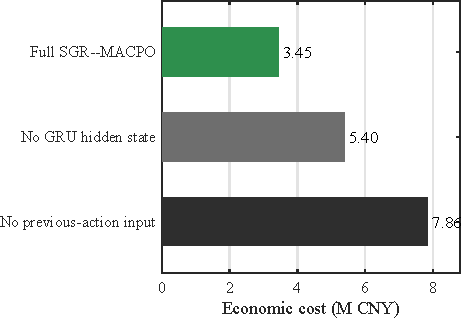
\includegraphics[width=0.98\columnwidth]{fig_recurrent_ablation_seed30.pdf}
  \caption{Same-checkpoint recurrent-information ablation in a representative evaluation scenario. Only the indicated temporal input is removed; all policy parameters and physical settings are otherwise unchanged.}
  \label{fig:recurrent_ablation}
\end{figure}

\FloatBarrier
\section{Discussion}
\label{sec:discussion}

The results connect each design element to an observable operating effect. The separate voltage-cost direction and backtracking tests produce an electricity-CDA clearing pattern and residual external balance that preserve active evening-peak coordination while avoiding the low-voltage event. In the hydrogen chain, internally cleared CDA quantities and regular external orders jointly form the in-transit inventory; explicit delivery timing then changes that inventory and feeds back to subsequent orders, storage, and electrolyzer operation even when the checkpoint is held fixed. The recurrent-information ablation further shows that both accumulated history and the previous action contribute to economical closed-loop behavior. Together, these results link the policy-update design, dual-market clearing, delayed physical state, and recurrent execution architecture to market, network, and multi-energy operation.

\section{Conclusion}
\label{sec:conclusion}

This paper presented \method for recurrent multi-agent scheduling of coupled electricity and hydrogen microgrids. The method combines decentralized GRU actors, centralized reward and voltage-cost critics, and a shared-system trust-region update with explicit recovery directions and sampled-cost backtracking. In the Env-v6 comparison, \method substantially reduces voltage violations relative to unconstrained MAPPO and obtains a more favorable economic trade-off than fixed-penalty MAPPO. The operating cases trace electricity CDA clearing to residual network exchange and trace the hydrogen CDA and regular external orders through the delayed delivery queue to storage and conversion. Removing either recurrent state or previous-action information markedly increases economic cost.

\section*{Data availability}

The Swiss-PDGs distribution-network data used in this study are publicly available at \url{https://github.com/aeonetos/Swiss-PDGs}. The environment configurations, trained checkpoints, and processed evaluation data underlying the reported results will be deposited in an open research repository; the persistent repository link will be inserted before submission. Until then, the processed data are available from the corresponding author on reasonable request.

\begin{thebibliography}{00}

\bibitem{yue2021hydrogen}
M. Yue, H. Lambert, E. Pahon, R. Roche, S. Jemei, D. Hissel, Hydrogen energy systems: A critical review of technologies, applications, trends and challenges, Renewable and Sustainable Energy Reviews 146 (2021) 111180. \url{https://doi.org/10.1016/j.rser.2021.111180}.

\bibitem{li2023hierarchical}
Q. Li, X. Xiao, Y. Pu, S. Luo, H. Liu, W. Chen, Hierarchical optimal scheduling method for regional integrated energy systems considering electricity-hydrogen shared energy, Applied Energy 349 (2023) 121670. \url{https://doi.org/10.1016/j.apenergy.2023.121670}.

\bibitem{he2025hydrogen}
W. He, C. Cai, Q.-L. Han, X. Qing, W. Du, F. Qian, Optimal scheduling of a hydrogen-based microgrid for an industrial park: A reinforcement learning approach, IEEE Transactions on Systems, Man, and Cybernetics: Systems 55 (6) (2025) 4348--4361. \url{https://doi.org/10.1109/TSMC.2025.3551325}.

\bibitem{paudel2019p2p}
A. Paudel, K. Chaudhari, C. Long, H.B. Gooi, Peer-to-peer energy trading in a prosumer-based community microgrid: A game-theoretic model, IEEE Transactions on Industrial Electronics 66 (8) (2019) 6087--6097. \url{https://doi.org/10.1109/TIE.2018.2874578}.

\bibitem{samadi2020decentralized}
E. Samadi, A. Badri, R. Ebrahimpour, Decentralized multi-agent based energy management of microgrid using reinforcement learning, International Journal of Electrical Power \& Energy Systems 122 (2020) 106211. \url{https://doi.org/10.1016/j.ijepes.2020.106211}.

\bibitem{fang2021multiagent}
X. Fang, Q. Zhao, J. Wang, Y. Han, Y. Li, Multi-agent deep reinforcement learning for distributed energy management and strategy optimization of microgrid market, Sustainable Cities and Society 74 (2021) 103163. \url{https://doi.org/10.1016/j.scs.2021.103163}.

\bibitem{zhang2023interconnected}
B. Zhang, W. Hu, A.M.Y.M. Ghias, X. Xu, Z. Chen, Multi-agent deep reinforcement learning based distributed control architecture for interconnected multi-energy microgrid energy management and optimization, Energy Conversion and Management 277 (2023) 116647. \url{https://doi.org/10.1016/j.enconman.2022.116647}.

\bibitem{glavic2017reinforcement}
M. Glavic, R. Fonteneau, D. Ernst, Reinforcement learning for electric power system decision and control: Past considerations and perspectives, IFAC-PapersOnLine 50 (1) (2017) 6918--6927. \url{https://doi.org/10.1016/j.ifacol.2017.08.1217}.

\bibitem{cao2020review}
D. Cao, W. Hu, J. Zhao, G. Zhang, B. Zhang, Z. Liu, Reinforcement learning and its applications in modern power and energy systems: A review, Journal of Modern Power Systems and Clean Energy 8 (6) (2020) 1029--1042. \url{https://doi.org/10.35833/MPCE.2020.000552}.

\bibitem{bahrami2021demand}
S. Bahrami, Y.C. Chen, V.W.S. Wong, Deep reinforcement learning for demand response in distribution networks, IEEE Transactions on Smart Grid 12 (2) (2021) 1496--1506. \url{https://doi.org/10.1109/TSG.2020.3037066}.

\bibitem{lowe2017maddpg}
R. Lowe, Y. Wu, A. Tamar, J. Harb, P. Abbeel, I. Mordatch, Multi-agent actor-critic for mixed cooperative-competitive environments, in: Advances in Neural Information Processing Systems 30, 2017, pp. 6379--6390.

\bibitem{foerster2018coma}
J. Foerster, G. Farquhar, T. Afouras, N. Nardelli, S. Whiteson, Counterfactual multi-agent policy gradients, Proceedings of the AAAI Conference on Artificial Intelligence 32 (1) (2018) 2974--2982. \url{https://doi.org/10.1609/aaai.v32i1.11794}.

\bibitem{schulman2017ppo}
J. Schulman, F. Wolski, P. Dhariwal, A. Radford, O. Klimov, Proximal policy optimization algorithms, arXiv:1707.06347, 2017. \url{https://doi.org/10.48550/arXiv.1707.06347}.

\bibitem{yu2022mappo}
C. Yu, A. Velu, E. Vinitsky, J. Gao, Y. Wang, A.M. Bayen, Y. Wu, The surprising effectiveness of PPO in cooperative multi-agent games, in: Advances in Neural Information Processing Systems 35, 2022, pp. 24611--24624. \url{https://doi.org/10.52202/068431-1787}.

\bibitem{gronauer2022survey}
S. Gronauer, K. Diepold, Multi-agent deep reinforcement learning: A survey, Artificial Intelligence Review 55 (2) (2022) 895--943. \url{https://doi.org/10.1007/s10462-021-09996-w}.

\bibitem{achiam2017cpo}
J. Achiam, D. Held, A. Tamar, P. Abbeel, Constrained policy optimization, in: Proceedings of the 34th International Conference on Machine Learning, Proceedings of Machine Learning Research 70, 2017, pp. 22--31.

\bibitem{gu2021macpo}
S. Gu, J.G. Kuba, M. Wen, R. Chen, Z. Wang, Z. Tian, J. Wang, A. Knoll, Y. Yang, Multi-agent constrained policy optimisation, arXiv:2110.02793, 2021. \url{https://doi.org/10.48550/arXiv.2110.02793}.

\bibitem{ma2025network}
Q. Ma, Z. Liu, Y. Ye, X. Liu, Network-constrained P2P trading: A safety-aware decentralized multi-agent reinforcement learning approach, IEEE Transactions on Smart Grid 16 (6) (2025) 5573--5588. \url{https://doi.org/10.1109/TSG.2025.3589888}.

\bibitem{liu2025carbon}
X. Liu, Y. Ye, S. Li, C. Zhang, Q. Ma, J. Zhu, Carbon-aware peer-to-peer energy trading in an unbalanced distribution network via a Nash equilibrium discovery deep reinforcement learning approach, IEEE Transactions on Smart Grid 16 (4) (2025) 3392--3405. \url{https://doi.org/10.1109/TSG.2025.3561515}.

\bibitem{hausknecht2015drqn}
M. Hausknecht, P. Stone, Deep recurrent Q-learning for partially observable MDPs, arXiv:1507.06527, 2015. \url{https://doi.org/10.48550/arXiv.1507.06527}.

\bibitem{vazquez2019demand}
J.R. V\'azquez-Canteli, Z. Nagy, Reinforcement learning for demand response: A review of algorithms and modeling techniques, Applied Energy 235 (2019) 1072--1089. \url{https://doi.org/10.1016/j.apenergy.2018.11.002}.

\bibitem{francois2018deep}
V. Fran\c{c}ois-Lavet, P. Henderson, R. Islam, M.G. Bellemare, J. Pineau, An introduction to deep reinforcement learning, Foundations and Trends in Machine Learning 11 (3--4) (2018) 219--354. \url{https://doi.org/10.1561/2200000071}.

\bibitem{staffell2019hydrogen}
I. Staffell, D. Scamman, A. Velazquez Abad, P. Balcombe, P.E. Dodds, P. Ekins, N. Shah, K.R. Ward, The role of hydrogen and fuel cells in the global energy system, Energy \& Environmental Science 12 (2) (2019) 463--491. \url{https://doi.org/10.1039/C8EE01157E}.

\bibitem{parra2019hydrogen}
D. Parra, L. Valverde, F.J. Pino, M.K. Patel, A review on the role, cost and value of hydrogen energy systems for deep decarbonisation, Renewable and Sustainable Energy Reviews 101 (2019) 279--294. \url{https://doi.org/10.1016/j.rser.2018.11.010}.

\bibitem{glenk2019economics}
G. Glenk, S. Reichelstein, Economics of converting renewable power to hydrogen, Nature Energy 4 (3) (2019) 216--222. \url{https://doi.org/10.1038/s41560-019-0326-1}.

\bibitem{almansoori2009supply}
A. Almansoori, N. Shah, Design and operation of a future hydrogen supply chain: Multi-period model, International Journal of Hydrogen Energy 34 (19) (2009) 7883--7897. \url{https://doi.org/10.1016/j.ijhydene.2009.07.109}.

\bibitem{moreno2017infrastructure}
M. Moreno-Benito, P. Agnolucci, L.G. Papageorgiou, Towards a sustainable hydrogen economy: Optimisation-based framework for hydrogen infrastructure development, Computers \& Chemical Engineering 102 (2017) 110--127. \url{https://doi.org/10.1016/j.compchemeng.2016.08.005}.

\bibitem{tushar2020p2p}
W. Tushar, T.K. Saha, C. Yuen, D. Smith, H.V. Poor, Peer-to-peer trading in electricity networks: An overview, IEEE Transactions on Smart Grid 11 (4) (2020) 3185--3200. \url{https://doi.org/10.1109/TSG.2020.2969657}.

\bibitem{sousa2019p2p}
T. Sousa, T. Soares, P. Pinson, F. Moret, T. Baroche, E. Sorin, Peer-to-peer and community-based markets: A comprehensive review, Renewable and Sustainable Energy Reviews 104 (2019) 367--378. \url{https://doi.org/10.1016/j.rser.2019.01.036}.

\bibitem{morstyn2018p2p}
T. Morstyn, N. Farrell, S.J. Darby, M.D. McCulloch, Using peer-to-peer energy-trading platforms to incentivize prosumers to form federated power plants, Nature Energy 3 (2) (2018) 94--101. \url{https://doi.org/10.1038/s41560-017-0075-y}.

\bibitem{sunehag2018vdn}
P. Sunehag, G. Lever, A. Gruslys, W.M. Czarnecki, V. Zambaldi, M. Jaderberg, M. Lanctot, N. Sonnerat, J.Z. Leibo, K. Tuyls, T. Graepel, Value-decomposition networks for cooperative multi-agent learning based on team reward, in: Proceedings of the 17th International Conference on Autonomous Agents and MultiAgent Systems, 2018, pp. 2085--2087.

\bibitem{rashid2020qmix}
T. Rashid, M. Samvelyan, C. Schroeder de Witt, G. Farquhar, J. Foerster, S. Whiteson, QMIX: Monotonic value function factorisation for deep multi-agent reinforcement learning, in: Proceedings of the 35th International Conference on Machine Learning, Proceedings of Machine Learning Research 80, 2018, pp. 4295--4304. \url{https://doi.org/10.48550/arXiv.1803.11485}.

\bibitem{hernandez2019survey}
P. Hernandez-Leal, B. Kartal, M.E. Taylor, A survey and critique of multiagent deep reinforcement learning, Autonomous Agents and Multi-Agent Systems 33 (6) (2019) 750--797. \url{https://doi.org/10.1007/s10458-019-09421-1}.

\bibitem{oroojlooy2023review}
A. Oroojlooy, D. Hajinezhad, A review of cooperative multi-agent deep reinforcement learning, Applied Intelligence 53 (11) (2023) 13677--13722. \url{https://doi.org/10.1007/s10489-022-04105-y}.

\bibitem{papoudakis2021benchmark}
G. Papoudakis, F. Christianos, L. Sch\"afer, S.V. Albrecht, Benchmarking multi-agent deep reinforcement learning algorithms in cooperative tasks, in: Advances in Neural Information Processing Systems 34, Datasets and Benchmarks Track, 2021. \url{https://doi.org/10.48550/arXiv.2006.07869}.

\bibitem{garcia2015safe}
J. Garc\'ia, F. Fern\'andez, A comprehensive survey on safe reinforcement learning, Journal of Machine Learning Research 16 (42) (2015) 1437--1480.

\bibitem{schulman2015trpo}
J. Schulman, S. Levine, P. Abbeel, M. Jordan, P. Moritz, Trust region policy optimization, in: Proceedings of the 32nd International Conference on Machine Learning, Proceedings of Machine Learning Research 37, 2015, pp. 1889--1897.

\bibitem{chow2018lyapunov}
Y. Chow, O. Nachum, E.A. Du\'e\~nez-Guzm\'an, M. Ghavamzadeh, A Lyapunov-based approach to safe reinforcement learning, in: Advances in Neural Information Processing Systems 31, 2018, pp. 8092--8101. \url{https://doi.org/10.48550/arXiv.1805.07708}.

\bibitem{tessler2019reward}
C. Tessler, D.J. Mankowitz, S. Mannor, Reward constrained policy optimization, in: Proceedings of the 7th International Conference on Learning Representations, 2019. \url{https://doi.org/10.48550/arXiv.1805.11074}.

\bibitem{ray2019benchmark}
A. Ray, J. Achiam, D. Amodei, Benchmarking safe exploration in deep reinforcement learning, arXiv:1910.01708, 2019. \url{https://doi.org/10.48550/arXiv.1910.01708}.

\bibitem{swisspdgs}
A. Eonetos, Swiss-PDGs: Swiss distribution grid data, GitHub repository. \url{https://github.com/aeonetos/Swiss-PDGs} (accessed 23 August 2026).

\bibitem{zimmerman2011matpower}
R.D. Zimmerman, C.E. Murillo-Sanchez, R.J. Thomas, MATPOWER: Steady-state operations, planning, and analysis tools for power systems research and education, IEEE Transactions on Power Systems 26 (1) (2011) 12--19. \url{https://doi.org/10.1109/TPWRS.2010.2051168}.

\end{thebibliography}

\balance

\end{document}
